\documentclass[11pt]{article}
\usepackage{xurl}
\usepackage{hyperref}
\usepackage{amsmath}
\usepackage{graphicx}
\hypersetup{colorlinks=true, linkcolor=blue, urlcolor=blue}
\usepackage{geometry}
% \usepackage{caption}
% \usepackage{subcaption}
\usepackage{subfig}
\setlength{\parindent}{0pt}

\title{\Huge Khidmat Report\\
\textit{WWF Bird Recognition Model}}
\author{Ali Hamza\\ ah05084
  \and
  Ali Haider Rizvi\\ ah05199
  \and
  M. Usaid Rehman\\ mr04302
}
\date{}  
\begin{document}
\maketitle
\begin{center}
    
\begin{figure}[h!]
    \centering
    \subfloat{{
\includegraphics[width=7cm]{./pictures/Hulogo.png} }}%
    \qquad
    \subfloat{{
\includegraphics[width=5cm]{./pictures/wwflogo.png} }}%
   % \caption{2 Figures side by side}%
    \label{fig:example}%
\end{figure}
\end{center}

\newpage
\tableofcontents
\newpage
\section{Introduction}
% Use first person plural (we, us) even if you did the Khidmat individually.
\subsection{Project Description}
\setlength{\parindent}{3em}
% An introduction of the project, no more than 2 sentences. Provide the highest level of detail only. Other details will come later.
% Typically, "This project is to <short description of porject> for/at <client>."
This project is aimed at creating and deploying a deep learning pipeline for WWF Pakistan to classify images of 
three different species of birds -- namely: common myna, house crow, and the house sparrow. This project 
would serve as a proof-of-concept for a larger model that WWF can use to classify a larger number of birds 
using a mobile application.

\subsection{About WWF Pakistan}
The World Wildlife Fund for Nature (WWF) is an international non-governmental organization
founded in 1961 that primarily works in the areas of wildlife conservation and preservation.
WWF also works in the domains of food security, renewable energy, ocean and forest preservation, 
and many others\footnote{\url{https://wwf.panda.org/}}.

WWF Pakistan is the Pakistan chapter of the World Wildlife Fund, working on similar problems as 
WWF International but in a more local context. WWF has more than five regional offices 
throughout the country, and has conducted several successful 
projects pertaining to freshwater conservation, water security, forests, climate change and others.
What they are most known for, however, is wildlife conservation --- the area that we 
have assisted WWF in.

\subsection{Project Background \& Context}
Keeping track of biodiversity is a challenge in Pakistan due to a lack of resources, personnel 
and governmental support. Pakistan has a plethora of wildlife and a rich and diverse ecosystem. 
WWF Pakistan has helped in the conservation of several endangered species such as the 
Indus River Dolphin and the Snow Leopard --- both of which are now experiencing a rise in numbers. 

However, wildlife preservation and protection extends beyond just the conservation of 
endangered species. Maintaining biodiversity is extremely important for 
wildlife protection and to maintain a healhty ecosystem and environment. Unfortunately, 
a lack of biodiversity is a major crisis that is unfolding across the globe. In order to 
combat this, it is imperative that researches have updated data about species populations, 
habitats, interactions etc. 

An important group of animals that contribute to biodiversity are birds. Therefore, 
it is vital that data pertaining to bird population is collected in Pakistan. 
To assist in this endeavor, WWF aims to enlist the help of citizen scientists who could 
help identify and locate birds and consequently update WWF's database. 

Our project aims to implement a deep learning pipeline that would 
classify images of three different species of birds --- house crow, common 
myna, and the house sparrow. The pipeline would take an image, preprocess it 
to a form that the model can work with, and then classify it using a deep 
neural network --- telling us what species the bird in the image belongs to. 

This pipeline serves as a proof-of-concept for a larger model that 
would be classifying hundreds of species of birds. This model will fit 
into a planned mobile application that citizen scientists can use to spot birds 
and then capture their image. Not only will the application classify the 
species of the bird but it will also update WWF's database, giving them 
access to more data about bird populations and their locations. 

The development of a larger deep learning model and an application is 
beyond the scope of our \textit{Khidmat} due to time restraints. 
We have succesfully implemented a computer vision pipeline for preprocessing 
and a deep neural network for classification for three species of birds.

\subsection{Work Plan}
\subsubsection{Project Description}
To create an algorithm that distinguishes between 3 birds that will act as the first stage in developing a larger ML model for the WWF app for recognizing birds.
\subsubsection{Expected Deliverables}
\
\begin{enumerate}
    \item Dataset on all 3 birds (Common Myna, Housecrow, Sparrow) 
    \item Machine Learning Model (Python Notebook)
    \item Validation and Training of Model
    \item Demonstration of Final Model 
    \item Report on Model, including Code, Explanations, and Documentation.
\end{enumerate}

\subsubsection{Planned Schedule}

\begin{itemize}
    \item [-] June Week 1: Images, Image Metadata, Relevance, Summary statistics, Scraped from Facebook, Instagram, Twitter, Datasets
    \item [-] June Week 2: Labelled data for training and testing. [Data in the proper format, ready to be used for the model]    
    \item [-] July Week 2: Prototype ML Model
    \item [-] July Week 3: Test run for the model using training data
    \item [-] July Week 4: Validation of model
    \item [-] August Week 1: Final training of reworked model 
    \item [-] August Week 2: Final Validation of reworked model
    \item [-] Sept Week 2: Demonstration of Model
    \item [-] Sept Week 4: Final Report and Delivery
\end{itemize}
\newpage % Start the report for each week on a new page.

% Copy-paste this section with necessary modifcations for each week.
\section{Weekly Work Log}
\subsection{\texttt{Week 1: }}
%Short Weekly Summary
\begin{center}
\begin{tabular}{|l|l|l|l|}
  \hline
  \textbf{Item} 	& \textbf{Activity} & \textbf{Time} & \textbf{ID} \\\hline
  1 & Scraped images for house sparrow & 2 & 05084 \\ \hline
  2 & Scraped images for house sparrow & 3 & 05084\\ \hline
  3 & Meeting with WWF & 1 & 05084\\ \hline
  4 & Scraped images for house crow & 2 & 05199\\ \hline
  5 & Scraped images for house crow & 1 & 05199\\ \hline
  6 & Scraped images for house sparrow & 2 & 05199\\ \hline
  7 & Meeting with WWF & 1 & 05084\\ \hline
  8 & Scraped Common Myna Pictures & 2 & 04302\\ \hline
  9 & Scraped Common Myna Pictures & 2 & 04302\\ \hline
  10 & Scraped Common Myna Pictures & 3 & 04302\\ \hline
  11 & Meeting with WWF & 1 & 05084 \\ \hline
\end{tabular}
    
\end{center}
The total time spent on the Khidmat this week is as follows.    
\begin{center}
    
\begin{tabular}{|l|c|}
  \hline
  \textbf{ID} & \textbf{Total Hours}\\\hline
  ah05084 & 6 \\\hline
  ah05199 & 6 \\\hline
  mr04302 & 8 \\\hline
\end{tabular}
\end{center}
\newpage
\subsection{\texttt{Week 2: }}
%Short Weekly Summary
\begin{center}
\begin{tabular}{|l|l|l|l|}
  \hline
  \textbf{Item} 	& \textbf{Activity} & \textbf{Time} & \textbf{ID} \\\hline
  1 & Analyzed the compiled dataset & 2.5 & 050584 \\ \hline
  2 & Wrote code for image preprocesing & 5 & 05084 \\ \hline
  3 & Internal Meeting & 1 & 05084 \\ \hline
  4 & Resized Images & 2.5 & 05199  \\ \hline
  5 & Coded Initial Model & 3.5 & 05199 \\ \hline 
  6 & Training and Tuning & 3.5 & 05199 \\ \hline
  7 & Internal Meeting & 1 & 05199 \\ \hline
  8 & Research Neural Nets & 1.5 & 04302 \\ \hline
  9 & Coded Initial Model & 3.5 & 04302 \\ \hline
  10 & Researched Optimization Methods & 1.5 & 04302 \\ \hline
  11 & Internal Meeting & 1 & 04302 \\ \hline
\end{tabular}
    
\end{center}
The total time spent on the Khidmat this week is as follows.    

\begin{center}
\begin{tabular}{|l|c|}
  \hline
  \textbf{ID} & \textbf{Total Hours}\\\hline
  ah05084 & 8.5 \\\hline
  ah05199 & 10 \\\hline
  mr04302 & 7.5 \\\hline
\end{tabular}
\end{center}

\subsection{\texttt{Week 3: }}
%Short Weekly Summary
\begin{center}
\begin{tabular}{|l|l|l|l|}
  \hline
  \textbf{Item} 	& \textbf{Activity} & \textbf{Time} & \textbf{ID} \\\hline
  1 & Worked on Model & 2 & ah05084 \\ \hline
  2 & Training and tuning & 2 & ah05084 \\ \hline
  3 & Worked on Report & 2 & ah05084 \\ \hline
  4 & Explored ResNet for better performance & 3 & ah05199 \\ \hline
  5 & Worked on Model & 2 & mr04302 \\ \hline
  6 & Training and tuning & 2 & mr04302 \\ \hline
\end{tabular}
    
\end{center}
The total time spent on the Khidmat this week is as follows.    

\begin{center}
\begin{tabular}{|l|c|}
  \hline
  \textbf{ID} & \textbf{Total Hours}\\\hline
  ah05084 & 6 \\\hline
  ah05199 & 3 \\\hline
  mr04302 & 4 \\\hline
\end{tabular}
\end{center}
\newpage
\subsection{\texttt{Week 4: }}
%Short Weekly Summary
\begin{center}
\begin{tabular}{|l|l|l|l|}
  \hline
  \textbf{Item} 	& \textbf{Activity} & \textbf{Time} & \textbf{ID} \\\hline
  
  1 & Shifted training to TPUs for faster training & 2.5 & 05199 \\ \hline
  2 & Training and Tuning & 11.5 & 05199 \\ \hline
  3 & Confusion Matrix/ Precision Recall & 1.5 & 05199 \\ \hline
\end{tabular}
    
\end{center}
The total time spent on the Khidmat this week is as follows.    
\begin{center}
\begin{tabular}{|l|c|}
  \hline
  \textbf{ID} & \textbf{Total Hours}\\\hline
  ah05084 & 0 \\\hline
  ah05199 & 15.5 \\\hline
  mr04302 & 0 \\\hline
\end{tabular}
\end{center}
\newpage
\subsection{\texttt{Week 5: }}
%Short Weekly Summar
\begin{center}
\begin{tabular}{|l|l|l|l|}
  \hline
  \textbf{Item} 	& \textbf{Activity} & \textbf{Time} & \textbf{ID} \\\hline
    1 & Scraped 40-50 images for all birds & 3 & 05084 \\ \hline
    2 & Worked on Intermediate Report & 3 & 05084 \\ \hline
    3 & Code Refactoring + Misc Google Colab work & 4 & 05084 \\ \hline
    4 & Worked on Neural Net + Github Syncing & 2.5 & 05084 \\ \hline
    5 & Worked on Intermediate Report & 3 & 04302 \\ \hline
\end{tabular}
    
\end{center}
The total time spent on the Khidmat this week is as follows.    
\begin{center}
\begin{tabular}{|l|c|}
  \hline
  \textbf{ID} & \textbf{Total Hours}\\\hline
  ah05084 & 12.5 \\\hline
  ah05199 & 0 \\\hline
  mr04302 & 3 \\\hline
\end{tabular}
\end{center}
\newpage

\subsection{\texttt{Week 6: }}
%Short Weekly Summary
\begin{center}
\begin{tabular}{|l|l|l|l|}
  \hline
  \textbf{Item} 	& \textbf{Activity} & \textbf{Time} & \textbf{ID} \\\hline
  1 & Training and Testing & 4 & 05084  \\ \hline
  2 & Worked on Intermediate Report & 2 & 05084 \\ \hline
  3 & Meeting with Dr. Sarah & 1 & 05084 \\ \hline
  4 & Meeting with Dr. Sarah & 1 & 04302 \\ \hline
  
\end{tabular}
    
\end{center}

The total time spent on the Khidmat this week is as follows.    
\begin{center}
\begin{tabular}{|l|c|}
  \hline
  \textbf{ID} & \textbf{Total Hours}\\\hline
  ah05084 & 7 \\\hline
  ah05199 & 0 \\\hline
  mr04302 & 1 \\\hline
\end{tabular}
\end{center}
\newpage
\subsection{\texttt{Week 7: }}
%Short Weekly Summary
\begin{center}
\begin{tabular}{|l|l|l|l|}
  \hline
  \textbf{Item} 	& \textbf{Activity} & \textbf{Time} & \textbf{ID} \\\hline
  1 & Cleaned Code & 2 & 05084 \\ \hline
  2 & Turned Notebook into Python Modules & 3 & 05084 \\ \hline
\end{tabular}
    
\end{center}
The total time spent on the Khidmat this week is as follows.    
\begin{center}
\begin{tabular}{|l|c|}
  \hline
  \textbf{ID} & \textbf{Total Hours}\\\hline
  ah05084 & 5 \\\hline
  ah05199 & 0 \\\hline
  mr04302 & 0 \\\hline
\end{tabular}
\end{center}
\newpage
\subsection{\texttt{Week 8: }}
%Short Weekly Summary
\begin{center}
\begin{tabular}{|l|l|l|l|}
  \hline
  \textbf{Item} 	& \textbf{Activity} & \textbf{Time} & \textbf{ID} \\\hline
  1 & Worked on Final Report & 8 & 05084 \\ \hline
  
\end{tabular}
    
\end{center}
The total time spent on the Khidmat this week is as follows.    
\begin{center}
\begin{tabular}{|l|c|}
  \hline
  \textbf{ID} & \textbf{Total Hours}\\\hline
  ah05084 & 8 \\\hline
  ah05199 & 0 \\\hline
  mr04302 & 0 \\\hline
\end{tabular}
\end{center}
\newpage
\section{Conclusion}
\newpage

\section{Technical Overview}
\subsection{Resources}
  The resources that we used for this project can be categorized into two main 
  categories: images, and technologies. Our first step was to acquire a set of images that would 
  function as our dataset. We collected around 550 images for each of the three 
  species of birds --- the house crow, common myna, and the house sparrow. We used 
  several different websites and online databases to find these images, we list 
  these websites below: 
  \begin{enumerate}
    \item \url{https://search.macaulaylibrary.org/catalog?taxonCode=myna&mediaType=p&q=Common\%20Myna}
    \item \url{https://ebird.org/media/catalog?taxonCode=commyn&mediaType=p&sort=rating_rank_desc&q=Common\%20Myna\%20-\%20Acridotheres\%20tristis}
    \item \url{https://ebird.org/media/catalog?taxonCode=houcro1&sort=rating_rank_desc&mediaType=p&regionCode=}
    \item \url{https://search.macaulaylibrary.org/catalog?taxonCode=houcro1&mediaType=p&region=Pakistan\%20(PK)&regionCode=PK&q=House\%20Crow\%20-\%20Corvus\%20splendens}
    \item \url{https://www.kaggle.com/gpiosenka/100-bird-species}
    \item \url{https://search.macaulaylibrary.org/catalog?taxonCode=houspa&mediaType=p&q=House\%20Sparrow}
    \item \url{https://ebird.org/media/catalog?taxonCode=houspa&mediaType=p&sort=rating_rank_desc&q=House\%20Sparrow\%20-\%20Passer\%20domesticus}
    \label{imagelinks}
  \end{enumerate}
  \setlength{\parskip}{1em}
  All collected images can be viewed at \url{https://drive.google.com/drive/folders/18k-roE_VJSB1dcrhvN1y_EosVF7Kb0dY?usp=sharing}.

  To preprocess our images, convert them into a usable dataset, and to create
  our deep learning model, we had to rely on several different preexisting tools.
  We list the tools that we used in this project below:
  \setlength{\parskip}{0em}
  \begin{itemize}
    \item \texttt{Python} --- The primary programming language that we used for this project.
      Most of the other tools that we used are different libraries \& modules for in Python.
    \item \texttt{OpenCV} --- A computer vision module in Python to preprocess the images. 
    \item \texttt{TensorFlow \& Keras} --- A Python library that we used to construct, and then 
      ttrain and test our neural network. 
    \item \texttt{Matplotlib} --- A plotting library for Python, which we used to visualize our
    \item \texttt{Sci-kit learn} --- A Python library for machine learning that we used to 
      construct our training and testing set. 
    \item \texttt{Google Colab} --- We used Colab notebooks to write code and then run code
      using GPU-accelerated computation that is made available using Google Colaboratory.
  \end{itemize}
 
\subsection{Overview of CS Techniques Used}
  This project was an amalgamation of several different aspects of computer science techniques.
  The process can be summarized into 5 main steps:
  \begin{enumerate}
    \item Image Collection
    \item Image Preprocessing 
    \item Construction of Neural Network 
    \item Training the Neural Network
    \item Testing and Optimization
  \end{enumerate}
  
  We briefly expand upon these steps in the following sections. For a more technical 
  description, please view the documentation (LINK HERE). 

  \subsubsection{Image Collection}
  We used the sources listed at~\ref{imagelinks} to collect images of the three species of birds.
  We downloaded approximately 650 images for each birds, which we then filtered
  down to around 550 to maintain uniform image quality. Based on our results, we believe
  the number of images that we have, i.e. the size of our dataset is adequate. 
  
  \subsubsection{Image Preprocessing}
  The next step was to pre-process these images to convert them into a
  usable dataset. 

 \begin{center}
    \begin{figure}[h!]
    \centering
    \subfloat{{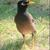
\includegraphics[width=0.25\textwidth]{./pictures/CM1.jpg}}}%
    \qquad
    \subfloat{{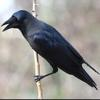
\includegraphics[width=0.25\textwidth]{./pictures/HC4.jpg} }}%
    \qquad
    \subfloat{{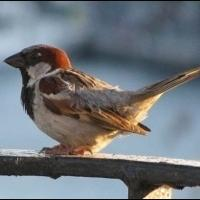
\includegraphics[width=0.25\textwidth]{./pictures/HS2.jpg} }}%

   \caption{Pictures of birds from the data set after preprocesing.}%
   \label{fig:birds}
    \end{figure}
  \end{center}

  \subsubsection{Neural Network Construction}
  Artificial neural networks form the basis for solving most artificial intelligence 
  problems. Image classification is one such problem. Neural networks represent connections 
  between artificial neurons, also called units. These connections are represented as weights 
  in the neural network. These weights are also called parameters and 
  learned by the neural network during supervised learning.

  There are several types of neural networks that are optimal for solving different 
  intelligence problems. Image recognition/classification has been solved using 
  several types of neural networks since the 1980s such as multilayer perceptrons. 
  A newer method to solve image classification problems (and problems generally 
  pertaining to computer vision) is the Convolutional Neural Network (CNN). 
  
  Unlike other neural networks, a CNN takes spatial information about the input image 
  into consideration during learning, allowing it to generally be more accurate. Therefore, 
  we decided to implement a CNN for this project. We first implemented a simplistic 
  CNN using two-dimensional convolutional layers that preexist in TensorFlow. However, 
  we found that our results were not as satisfactory as we hoped for them to be.

  We then tried implementing the Residual Neural Network (ResNet), which is built
  upon the same idea as CNNs but significantly improves accuracy and performance. 
  ResNet utilize skip connections or shortcuts between layers. Specifically, we leveraged 
  TensorFlow's built-in ResNet50 implementation, a variant of ResNet that utilizes 
  48 convolutional layers, a MaxPool layer and an Average Pool layer. However, since 
  ResNet50 is a fairly deep architecture which is more useful when implementing models 
  for data sets that are quite large, with at least several thousand examples.

  Therefore, we resorted to the CNN once again since it was more suited to 
  our data set.
  For more technical information on the neural network construction, please see <LINK>.
  
  \subsubsection{Training the Neural Network}
  To train neural networks, there are several different methods that optimize 
  the cost function. The most famous of these is the stochastic gradient descent (SGD). 
  SGD is a stochastic approximation of the simpler gradient descent optimization. Gradient 
  descent approximates the gradient for the entire training set at each iteration. However, 
  stochastic gradient descent approximates the gradient for one example in the training set 
  per iteration --- making it much faster. 

  A newer method called minibatch stochastic gradient finds the middle ground between 
  gradient descent and SGD. It approximates the gradient in each iteration using a randomly 
  selected minibatch of training examples. These minibatches are also effective for 
  parellel computation using TPUs. 

  We used the Adaptive Moment Estimation or \textit{Adam} optimization algorithm. Adam is an 
  effective algorithm for problems with sparse gradients such as computer vision problems. 
  This optimization algorithm relies on three hyperparameters: $\alpha, \beta_1, \beta_2 $, and $\epsilon$.
  Adam is very effective in optimizing problems that contains a large number 
  of trainable parameters. The value we set for $\alpha$ was 0.001 and the $\beta$ values 
  were set as default, i.e. 0.9 and 0.999. The loss function for our model was 
  the cross-entropy loss function which is quite popular in image classification tasks.
   
  \subsection{Results}
  To train our neural network, we ran the optimization algorithm on it for 
  110 epochs, and we kept the minibatch size as 64, in order to not overburden the TPU.
  At the end of training, our accuracy reached approximately 86\% and our loss value 
  was reduced to almost 0.67 as shown in Figure~\ref{fig:results}.

  Other than just the accuracy and loss metrics, we used the confusion matrix to 
  analyze the performance of our model. The confusion matrix is a standard for
  judging the performance of a model in a classification problem. Our confusion 
  matrix looked like this:
  \[\begin{bmatrix}
    117 & 15 & 9 \\
    13 & 134 & 6 \\
    14 & 14 & 128
 \end{bmatrix}\]
 \vspace{-2 em}
 \begin{center}
      \begin{figure}[h!]
    \centering
    \subfloat{{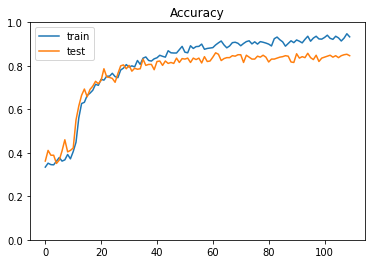
\includegraphics[width=0.45\textwidth]{./pictures/Acc_finalmodel.png}}}%
    \qquad
    \subfloat{{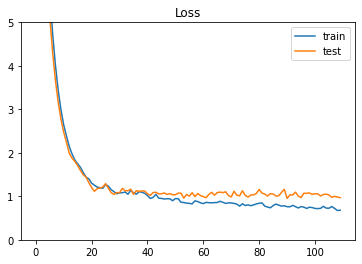
\includegraphics[width=0.45\textwidth]{./pictures/loss_finalmodel.png} }}%
   \caption{Plots for the accuracy and loss resulting from training the CNN.}%
   \label{fig:results}
\end{figure}
\end{center}
\vspace{-2 em}
Lastly, we also calculated the accuracy, precision, recall, and F1 scores. Our accuracy score was almost
0.8222, precision was 0.84209, recall was 0.842039, and F1 score was 0.8417. Therefore, 
considering the small data set, our model did do reasonably well in terms of performance.

\section{Conclusion}%
\label{sec:conclusion}
Our \textit{Khidmat} Project is the starting step for a larger model that should be able 
to identify many more species of birds commonly found in Pakistan. This will clearly make
the data set much larger. One of the primary challenges we faced was that our data set was fairly
small. An improvement that we would suggest would be to use a much larger data set. This data 
set can be accumulated using web scraping. Ideally, there should be several thousand 
images for each birds. Not only does this have the potential of improving accuracy but it also 
allows for better, more complex architectures to be used such as DenseNet and ResNet.
We would also recommend tweaking the existing model more and adjusting hyperparameters in 
order to find a better configuration that optimizes the model the most.

This project was a great learning experience for us and we are thankful to WWF Pakistan, 
especially Mr. Jamshed Iqbal for letting us be a part of the great work that WWF Pakistan does 
for animal conservation. We are also thankful to our internal supervisor, Dr. Sarah Hasnain, 
for letting us know of this opportunity and for supporting us throughout the project.

\newpage
\appendix
% Show your external supervisor your report, especially the weekly upates; have them sign a printed copy of this page; scan the signed page; and include the scanned page in this document as an image.
\section{Documentation}
\begin{itemize}
  \item \texttt{load$\_$dataset(size)}
  This function has been designed to take in the size of the images being used for training, each image being a square. The function will then return a list of images, and labels for training. The dataset variable returns a list of paths for the images, and a the labels variable returns list of labels for those images.
  \item \texttt{read$\_$image(dataset)}
  \item This takes the dataset variable as an argument and returns a list of images that have been turned where each image is represented by a list of RGB values for each pixel in the image.
  \item \texttt{create$\_$model()}
\end{itemize}
\newpage
\begin{center}
  {\Large\bf Khidmat Completion Form}\\[5pt]
  \small To be completed by the external supervisor.  
\end{center}
\bigskip

\noindent{\it Please use the space below to provide any comments you may have on the students' 
performance, the Khidmat program, or any other feedback you want to share with Habib 
University's Khidmat committee. We can also be reached 
at \href{mailto:khidmat@sse.habib.edu.pk}{khidmat@sse.habib.edu.pk}.}
\vfill

\begin{center}
  \rule{.8\textwidth}{.5pt}
\end{center}
\medskip

% Insert your name below.

I hereby certify that I supervised XXX and XXX for the Khidmat described in this report. 
Furthermore, that I have read and agree with the weekly updates included in this report.
My signature below marks the successful completion of the work undertaken for the Khidmat.\\
\bigskip
\bigskip

\noindent\begin{tabular}{@{}p{.6\textwidth}@{\hspace{.1\textwidth}}p{.3\textwidth}}
  \hrulefill \&   \hrulefill\\
  Name and signature & Location and date
\end{tabular}

\medskip\end{document}
